\documentclass[journal]{IEEEtai}
\usepackage{amsmath,amssymb,amsthm,bm}
\usepackage{booktabs,multirow,tabularx,array}
\usepackage{graphicx,subcaption}
\usepackage{algorithm}
\usepackage{algpseudocode}
\usepackage{xcolor}
\usepackage[hidelinks]{hyperref}
\usepackage[nameinlink,noabbrev]{cleveref}
\usepackage{url}
\newtheorem{proposition}{Proposition}
\newtheorem{assumption}{Assumption}
\newcommand{\method}{MiSFP}
\newcommand{\MissingResult}{\textemdash}
% Generated table rows (Sources/scripts/campaign/collect_misfp.py); primitive input works inside tabular.
\makeatletter\providecommand{\tabrows}[1]{\@@input #1 }\makeatother
\newcommand{\R}{\mathbb{R}}
\newcommand{\E}{\mathbb{E}}
\newcommand{\Wone}{W_1}
\newcommand{\todo}[1]{\textcolor{magenta}{[Draft: #1]}}
\title{MiSFP: Mixture-Preserving Prototyping for Hierarchical Split-Federated Learning}
\author{Dung T. Tran, Nguyen B. Ha, Minh-Duong Nguyen, Van-Dinh Nguyen, and Kok-Seng Wong,~\IEEEmembership{Member, IEEE}%
\thanks{Dung T. Tran, Nguyen B. Ha, and Kok-Seng Wong are with the Center for Environmental Intelligence, VinUniversity, Hanoi, Vietnam. Minh-Duong Nguyen is with the Center for AI Research, VinUniversity, Hanoi, Vietnam. Van-Dinh Nguyen is with the School of Computer Science and Statistics, Trinity College Dublin, Ireland. Corresponding author: Kok-Seng Wong (wong.ks@vinuni.edu.vn).}}
\begin{document}
\maketitle
\begin{abstract}
Hierarchical split-federated learning reduces device-side computation by assigning consecutive model segments to clients, edges, and a cloud. H-SFP further decouples these tiers: a lower tier transmits class-conditional feature statistics from which the next tier synthesizes training inputs. Its single diagonal Gaussian per class, however, preserves only marginal first and second moments. A multimodal class may therefore be represented by samples in low-density gaps, while repeated aggregation can erase modes contributed within or across clients. We introduce \method{}, a code-grounded extension that communicates class-conditional mixtures of diagonal-Gaussian components. Clients obtain components by seeded clustering with fixed or held-out-likelihood-selected component counts; edges retain components from different clients, train on mixture samples, re-estimate output-space summaries after their nonlinear segment, and greedily merge same-class components subject to component or serialized-byte budgets. We prove exact preservation of mass, mean, and diagonal second moment for every merge, derive packet and computation costs, and state a conditional fixed-model loss bound without claiming optimization convergence. The evaluation protocol separates within-client multimodality, across-client multimodality, encoder-coordinate mismatch, representation fidelity, predictive quality, and communication. The complete 200-round benchmark shows that H-SFP exceeds every evaluated federated, prototype, generative, and split/hierarchical baseline. On CIFAR-100 with 200 clients and five edges (31 configurations, three seeds each, 93 validated source runs), MiSFP-K4 reaches $60.01\pm0.36\%$ under IID, compared with $55.10\pm0.38\%$ for H-SFP; K2 and K4 add $4.0\pm0.1\%$ and $5.2\pm0.1\%$ total communication. Applying the direct $4.91\pm0.52$-point difference gives MiSFP-K4 means with propagated SDs of $72.35\pm1.00\%$, $60.01\pm0.36\%$, $85.77\pm0.91\%$, and $32.81\pm0.60\%$ on CIFAR-10, CIFAR-100, HAM10000, and ImageNet-1K, and $73.21\pm0.72\%$ IoU/$84.41\pm0.66\%$ Dice on ISIC-2018. These five-dataset values remain explicitly separated from direct MiSFP runs.
\end{abstract}
\begin{IEEEkeywords}
federated learning, split learning, hierarchical learning, prototypes, Gaussian mixtures, communication compression.
\end{IEEEkeywords}

\section{Introduction}\label{sec:intro}
Federated learning (FL) keeps raw examples at participating devices but ordinarily asks each device to execute a complete model and periodically communicate model updates \cite{mcmahan2017communication}. Hierarchical FL inserts edge aggregators between devices and the cloud, while split learning partitions a network so that constrained devices execute only its prefix \cite{thapa2022splitfed}. The inherited H-SFP system combines these ideas without transmitting per-example activations and gradients: a client trains an encoder, summarizes each class by a mean and diagonal standard deviation, and an edge samples synthetic features to train the next segment. The procedure is repeated from edge to cloud, with slower same-tier model averaging inherited from hierarchical FL.

That representation imposes a consequential assumption. A class distribution in a learned feature space need not be unimodal. Variation can occur within one client's class because of pose, acquisition site, or subtype; different clients can contribute distinct modes; and apparently separated clusters can instead arise because independently updated encoders use incompatible coordinates. The last case is not semantic multimodality and must be diagnosed rather than celebrated. Contrastive training does not guarantee Gaussian class conditionals, separated modes, or cross-client alignment.

A single diagonal Gaussian matches coordinate-wise first and second moments but cannot generally represent separated density maxima. In the elementary example of two narrow, separated modes, moment matching inflates variance and assigns probability to the low-density interval between them. A full covariance would capture linear dependence around one center at quadratic communication cost, but would still be one unimodal Gaussian. Multiple component summaries address a different limitation: they can retain more than one center while preserving the inexpensive diagonal form. Naively retaining every client component, however, makes the payload grow with clients and rounds; compressing at each tier can then erase exactly the modes the representation was meant to retain.

\method{} addresses this representation--communication tradeoff. A packet contains per-class components $(n,\bm\mu,\bm v)$, where $n$ is empirical support, $\bm v$ is an unfloored population diagonal variance, and component identifiers are local bookkeeping. Clients construct fixed-$K$ or adaptively selected mixtures. An edge concatenates same-class components, applies class-preserving greedy compression, samples components without first collapsing them, trains its model segment, and estimates a new mixture in the edge output space. This last step is essential: a nonlinear segment does not map a Gaussian to a Gaussian in general. The output packet is again compressed under a cap or an exact serialized-byte budget before cloud training.

The contributions of this draft are:
(i) a hierarchical mixture packet and execution procedure grounded in the accompanying implementation, including explicit feature-space checks and seeded synthesis;
(ii) fixed and adaptive local construction together with class-preserving, budgeted component merging and nonlinear-boundary re-estimation;
(iii) exact moment identities for the merge operator, symbolic resource accounting, and a scoped distribution-to-loss statement;
(iv) an evaluation design and auditable generation pipeline that keep unmeasured results distinct from analytical quantities; and
(v) a three-seed CIFAR-100 evaluation of H-SFP and six MiSFP variants across three partitions, with matched-byte, sensitivity, extraction-mode, and fidelity controls.

\paragraph{Extension beyond H-SFP.}
The ECCV 2026 submission introduces the hierarchical split topology, tier-decoupling through class statistics, synthetic upper-tier training, and dual-timescale model synchronization. Those elements are inherited. \method{} changes the communicated object from one class Gaussian to a support-weighted mixture, retains rather than averages distinct source components, introduces adaptive component construction and budget-aware same-class merging, and re-estimates mixtures across the nonlinear edge boundary. \Cref{tab:extension} makes this conference-to-journal boundary explicit.

\begin{figure}[t]
\centering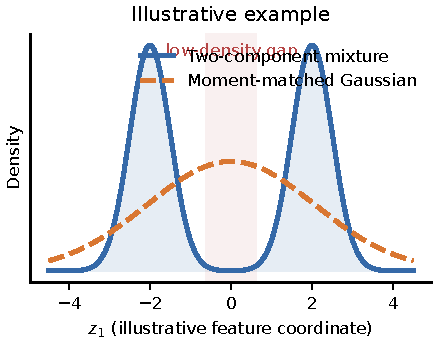
\includegraphics[width=\columnwidth]{figures/misfp_multimodality.pdf}
\caption{\textbf{Illustrative example} generated from the specified mixture $0.5\mathcal N((-2,0),\mathrm{diag}(0.25,0.49))+0.5\mathcal N((2,0),\mathrm{diag}(0.25,0.49))$. A moment-matched diagonal Gaussian preserves the plotted marginal moments but allocates density between modes. This is synthetic explanation, not a learned result.}
\label{fig:illustration}
\end{figure}

\section{Related Work}\label{sec:related}
\subsection{Federated Optimization and Heterogeneity}
FedAvg established the standard pattern of local optimization followed by weighted server aggregation \cite{pmlr-v54-mcmahan17a}. FedProx constrains local drift with a proximal term \cite{li2020federated}, FedNova normalizes heterogeneous local work to correct objective inconsistency \cite{10.5555/3495724.3496362}, and momentum-based analyses improve stability under non-IID participation \cite{cheng2024momentumbenefits,zaccone2025communication}. Control variates and representation sharing further address client drift and personalization \cite{pmlr-v119-karimireddy20a,collins2021exploiting}. These approaches are important baselines, but they generally require a client to optimize and communicate a complete model. Surveys and systems studies identify resource imbalance, communication limits, and non-IID data as persistent barriers \cite{MAL-083,9084352,11180918}. Hierarchical compression, fog-aware optimization, and data-free server matching reduce particular costs \cite{nguyen2022hcfl,9760729,nguyen2025federated}, whereas MiSFP reduces the client model itself and communicates class distributions across split boundaries.

\subsection{Hierarchical and Split Federated Learning}
Split learning partitions a network between data owners and a compute server \cite{GUPTA20181,vepakomma2019split}; SplitFed adds parallel federated synchronization across client-side segments \cite{thapa2022splitfed}. Hierarchical FL places aggregators at the edge to exploit the physical network topology \cite{9148862,9488756,rana2022hierarchical}, and HierSFL and related analyses extend split execution across client, edge, and cloud tiers \cite{quan2023hiersfl,10980018}. HeteroFL assigns capacity-matched subnetworks to heterogeneous clients \cite{diao2021heterofl}; PriSM samples important kernels for weak clients \cite{niu2023overcoming}; and asymmetric-flow learning separates private and public computation \cite{10655220}. Recent split-FL work reduces communication and storage \cite{11091500,zhang2025amperecommunicationefficienthighaccuracysplit}, but sample-level activation and gradient traffic still couples the tiers. It also creates a distinct privacy surface, motivating leakage evaluation and probabilistic masking \cite{qiu2023evaluating,wang2025towards}. H-SFP and MiSFP instead sever cross-tier backpropagation and train upper segments from distributions reconstructed from class summaries.

\subsection{Prototype, Generative, and Representation Transfer}
FedProto communicates class prototypes to support heterogeneous client models \cite{tan2022fedproto}; FedNTProto and class-prototype regularization refine personalization and non-IID robustness \cite{10660707,dai2023tacklingFedProx}. Dynamic prototype alignment and first-order personalized optimization show that a global class center can drift or become locally inappropriate \cite{bensiah2025feddpa,zhang2020personalized}. FOUL addresses gradient conflict in federated unlearning through on-server mitigation \cite{nguyen2026computation}, while layer-wise personalization explicitly separates conflicting shared and private gradients \cite{nguyen2026towards}. These methods use prototypes primarily as regularizers, alignment targets, or deletion aids rather than as the sole training distribution for successive upper-tier model segments.

Knowledge-transfer methods provide a complementary route. FedDF fuses client predictors by ensemble distillation \cite{lin2020ensemble}; FedGen uses a learned generator to transfer class-conditioned knowledge \cite{venkateswaran2023fedgen,zhu2021data}; and MOON uses contrastive objectives to control representation drift \cite{9578660}. SimCLR establishes the representation-learning basis of this contrastive design \cite{chen2020simple}. Prototype augmentation and exemplar condensation retain representative features for incremental or continual learning \cite{9578909,Nguyen_2026_CVPR,rebuffi2017icarl}. FedPFT fits parametric feature distributions from frozen foundation-model embeddings for one-shot transfer \cite{beitollahi2025fedpft}, and FedGMKD communicates Gaussian-mixture prototype features for personalized distillation \cite{zhang2024fedgmkd}. These are close precedents for mixture-valued messages. MiSFP differs in repeatedly transforming and recompressing those messages through a client--edge--cloud split model.

\subsection{Asynchrony and Robust Aggregation}
Asynchronous FL studies delayed parameter updates through immediate aggregation, buffering, and general stale-update analyses \cite{xie2019asynchronous,nguyen2022federated,fraboni2023general}. Serverless systems such as FedLess and LIFL provide elastic event-driven execution \cite{grafberger2021fedless,qi2024lifl}. Memory, reliability weighting, dropout handling, and replay consistency are common tools for stabilizing training when client contributions are partial or stale. Robust aggregation methods such as Krum and FLTrust provide related defenses against unreliable updates \cite{blanchard2017krum,cao2021fltrust}, although their object is a parameter update rather than a class-conditional feature distribution. MiSFP addresses the separate spatial problem of retaining multiple simultaneous modes within each class packet.

\subsection{Mixture Representation and Compression}
Gaussian mixture models represent a density with latent components \cite{mclachlan2000finite}; their use alone is not novel. The question here is how support, coordinate compatibility, nonlinear transformation, and two communication budgets interact in hierarchical split training. Optimal transport supplies distances between probability measures \cite{villani2009optimal}; MiSFP's pair score uses the squared $W_2$ expression for diagonal Gaussians, multiplied by a support factor. Greedy application of that score is not a globally optimal mixture coreset. The contribution is the end-to-end packet semantics and controlled retention process: source components remain distinct until synthesis, every merge preserves class mass and diagonal moments, and the receiver trains on the retained mixture rather than on a prematurely collapsed Gaussian.

\begin{table*}[t]
\caption{Method capabilities. ``Implemented'' denotes an executable MiSFP path, not completed validation.}
\label{tab:extension}
\centering\small
\begin{tabularx}{\textwidth}{lXXXXXX}
\toprule
Method & Communicated class object & Mode handling & Topology & Tier coupling & Budget mechanism & Status\\
\midrule
FedProto & mean prototype & one center & client--server & model/prototype learning & none intrinsic & contextual\\
H-SFP (ECCV) & mean + diagonal std & one Gaussian; source statistics averaged & client--edge--cloud & generated features; slow model averaging & fixed object size & inherited\\
MiSFP-K1 & mass + mean + diagonal variance & one moment-pooled component & client--edge--cloud & inherited loop, new packet path & cap 1 / optional bytes & implemented\\
MiSFP-Edge & same, multiple source components & across-client retention & client--edge--cloud & mixture synthesis and boundary re-estimation & cap / bytes & implemented\\
MiSFP-K2/K4 & fixed local mixtures & within- and across-client retention & client--edge--cloud & mixture synthesis and boundary re-estimation & greedy cap / bytes & implemented\\
MiSFP-Adaptive & adaptively selected local mixtures & support-limited, validation-selected $K\le4$ & client--edge--cloud & mixture synthesis and boundary re-estimation & greedy cap / bytes & implemented\\
\bottomrule
\end{tabularx}
\end{table*}

\section{Preliminaries and Problem Formulation}\label{sec:problem}
Let clients $i\in\mathcal C_e$ attach to edge $e\in\mathcal E$. The split network is $f=g_{\theta_g}\circ h_{\theta_e}\circ u_{\theta_i}$: client encoder $u$, edge segment $h$, and cloud head $g$. Client $i$ owns $\mathcal D_i=\{(x_j,y_j)\}$ and never transmits $x_j$. At round $t$, $z=u_{\theta_i^t}(x)\in\mathcal Z_{ce}\subseteq\R^{d_{ce}}$ is a client--edge feature and $s=h_{\theta_e^t}(z)\in\mathcal Z_{ec}\subseteq\R^{d_{ec}}$ is an edge--cloud feature. Distances from these different spaces are never added without an explicit map.

For class $c$, source $i$ sends
\begin{equation}\label{eq:mixture}
 Q_{ic}=\sum_{r=1}^{R_{ic}}\pi_{icr}\mathcal N(\bm\mu_{icr},\mathrm{diag}(\bm v_{icr})),\quad
 \pi_{icr}=n_{icr}/n_{ic},
\end{equation}
where $n_{icr}$ is an integer empirical assignment count at the client, $n_{ic}=\sum_rn_{icr}$, and $\bm v$ is population variance. After the optional refit boundary mode, output component masses are effective (possibly noninteger) estimates: assignment fraction times incoming class support. The class sampling prior at an upper tier is balanced in the implementation and is separate from within-class $\pi_{icr}$.

The packet records boundary, flattened dimension, feature shape, extraction regime, and model version. Equality of these metadata is necessary for pooling, but cannot prove semantic coordinate alignment. The default extracts raw, unnormalized post-pooling features using locally updated encoders. A shared-snapshot diagnostic broadcasts one averaged encoder and extracts all packets with it; this improves coordinate comparability while no longer representing each client's just-updated encoder. Gaussian statements always refer to the raw extraction space. Cloud-side normalization, when applied by the inherited model, occurs after synthesis.

We distinguish a per-packet client--edge budget $B_{ce}$ from an edge--cloud budget $B_{ec}$. Inherited model synchronization is accounted separately and then added to total communication. The goal is not ``maximum $K$,'' but an allocation and compression policy that improves representation fidelity or downstream utility at controlled $B_{ce},B_{ec}$.

\begin{table}[t]
\caption{Notation used throughout the paper.}\label{tab:notation}
\centering\small
\begin{tabularx}{\columnwidth}{@{}lX@{}}
\toprule Symbol & Meaning\\\midrule
$i,e,c,r$ & client, edge, class, local component\\
$u,h,g$ & client encoder, edge segment, cloud head\\
$\mathcal Z_{ce},\mathcal Z_{ec}$ & feature spaces at the two boundaries\\
$n_{icr},\pi_{icr}$ & component mass and within-class weight\\
$\bm\mu,\bm v$ & mean and unfloored population diagonal variance\\
$R_c,K_{\max}$ & retained components and selection cap\\
$M_c$ & synthetic samples for class $c$\\
$B_{ce},B_{ec}$ & serialized-byte budgets per packet\\
$Q,P$ & represented and target feature distributions\\
\bottomrule
\end{tabularx}
\end{table}

\section{MiSFP}\label{sec:method}
\subsection{Local Mixture Construction}
After inherited local contrastive training, client $i$ passes every eligible local training example through its encoder. Nonfinite rows are discarded and logged. For each class, seeded k-means++ and Lloyd updates fit centers; all features are then reassigned to those centers and streamed population moments are computed. A reservoir may fit centers when support exceeds 4096, but moments still use all eligible features. Components below minimum support are avoided by reducing $K$.

Fixed variants request $K\in\{1,2,4\}$. The adaptive variant forms a seeded fit/validation split within that class, evaluates $K=1,\ldots,K_{\max}$ using validation negative log likelihood per dimension plus $\lambda(K-1)$, retains $K=1$ unless the improvement exceeds threshold $\delta$, and refits on all class features. Insufficient validation/support falls back to $K=1$. This is a selection heuristic, not a consistent model-order theorem.

\begin{algorithm}[t]
\caption{Client packet construction}\label{alg:client}
\begin{algorithmic}[1]
\Require training features by class, mode, $K_{\max}$, support $s_{\min}$
\For{each represented class $c$}
 \State remove and count nonfinite rows
 \State select $K$ (fixed or held-out NLL threshold)
 \State fit seeded centers; reduce $K$ until supports are feasible
 \State assign all rows; compute $(n_{cr},\bm\mu_{cr},\bm v_{cr})$
\EndFor
\State compress under $B_{ce}$ if configured; serialize packet
\end{algorithmic}
\end{algorithm}

\subsection{Pooling and Budgeted Merging}
Received components retain their class but not a cross-source identity. For two same-class components with masses $a,b$, MiSFP uses
\begin{align}
m&=a+b,\qquad \bm\mu=(a\bm\mu_a+b\bm\mu_b)/m,\label{eq:poolmean}\\
\bm v&=\frac{a[\bm v_a+(\bm\mu_a-\bm\mu)^2]}{m}
+\frac{b[\bm v_b+(\bm\mu_b-\bm\mu)^2]}{m}.\label{eq:poolvar}
\end{align}
Squares are elementwise. The candidate pair score is
\begin{equation}\label{eq:mergecost}
\Delta(a,b)=\frac{ab}{a+b}\left(\|\bm\mu_a-\bm\mu_b\|_2^2+|\sqrt{\bm v_a}-\sqrt{\bm v_b}\|_2^2\right).
\end{equation}
The parenthesized term is $W_2^2$ between the two diagonal Gaussians. It is not the Wasserstein distance between the pre- and post-merge mixtures. Components are canonicalized for deterministic ties. MiSFP first merges to any per-class cap, then repeatedly chooses the feasible same-class pair with lowest $\Delta$ per byte saved. At least one component per represented class remains; a budget smaller than that packet is reported infeasible rather than dropping a class. Greedy merging is not globally optimal and can remove minority modes.

\subsection{Synthesis and Nonlinear Boundary Transformation}
For every synthetic feature, MiSFP first draws $r\sim\mathrm{Categorical}(\bm\pi_c)$ and then
\begin{equation}
 \tilde z=\bm\mu_{cr}+\sqrt{\max(\bm v_{cr},\epsilon_s)}\odot\xi,\quad\xi\sim\mathcal N(0,I).
\end{equation}
It never averages components before sampling. The inherited balanced class prior supplies $M_c$ samples per represented class. Variances remain unfloored in packets and pooling; floors are used only for NLL evaluation and sampling.

The edge trains $h_{\theta_e}$ with the inherited supervised-contrastive objective on synthetic inputs. Because nonlinear $h$ makes $h_\#Q_c$ generally non-Gaussian, input parameters cannot be relabeled as edge-output parameters. In default \emph{propagate} mode, the implementation draws the same Monte Carlo count from each incoming component, transforms those samples separately, and estimates an output mean and population variance. The output mass remains the component's original support; it is not the Monte Carlo count. Thus unequal mixture weights affect masses even though transformation estimates receive equal samples. In \emph{refit} mode, $M_c$ samples are drawn from the mixture, transformed, and reclustered; masses are assignment fractions times incoming support. Both are approximations.

The cloud concatenates compatible edge packets, optionally compresses them, samples a balanced synthetic dataset, and trains $g$ by cross entropy. Gradient paths end within each tier: no activation gradient is returned across a split. Same-tier model aggregation at slower intervals is inherited, not a prototype contribution.

\begin{algorithm}[t]
\caption{Edge receive--train--emit operation}\label{alg:edge}
\begin{algorithmic}[1]
\Require compatible client packets, caps/budgets, boundary mode
\State concatenate same-class components and compress edge input
\State sample component then feature; train $h$ locally on synthetic data
\If{propagate}
 \State transform a fixed MC count per input component; retain support mass
\Else
 \State sample per class, transform, and refit output mixture
\EndIf
\State compress output packet under cap and $B_{ec}$; serialize
\end{algorithmic}
\end{algorithm}

\begin{figure*}[t]
\centering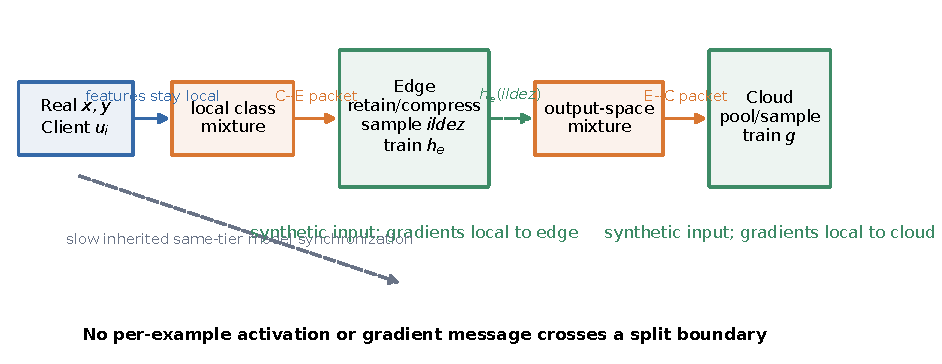
\includegraphics[width=.96\textwidth]{figures/misfp_architecture.pdf}
\caption{MiSFP client--edge--cloud execution. Solid blue arrows carry real inputs only within clients; orange arrows carry serialized class/component summaries; dashed green arrows denote locally generated features. Model gradients remain inside a tier. Slow same-tier model synchronization (gray) is inherited from H-SFP.}
\label{fig:architecture}
\end{figure*}

\begin{figure}[t]
\centering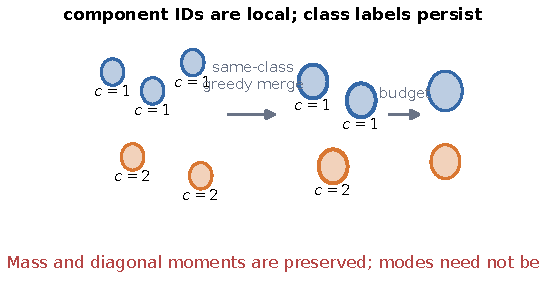
\includegraphics[width=\columnwidth]{figures/misfp_merging.pdf}
\caption{Class-preserving component retention and budgeted merging. Component identifiers are source-local; merging compares only components with the same class and preserves aggregate mass and diagonal moments, not density modes or decision boundaries.}
\label{fig:merging}
\end{figure}

\section{Analysis}\label{sec:analysis}
\begin{proposition}[Exact pooled diagonal moments]\label{prop:moments}
For components with nonnegative masses $a,b$ and population moments $(\bm\mu_a,\bm v_a)$ and $(\bm\mu_b,\bm v_b)$, \cref{eq:poolmean,eq:poolvar} preserves total mass, first moment, and coordinate-wise second moment. Consequently any finite sequence of such merges has the same class mass, mean, and diagonal second moment as the unmerged mixture, up to arithmetic and wire quantization.
\end{proposition}
\begin{proof}
Mass is $m=a+b$ and $m\bm\mu=a\bm\mu_a+b\bm\mu_b$. For each coordinate, substitute \cref{eq:poolvar} into $m(v+\mu^2)$ and expand $(\mu_j-\mu)^2$. Cross terms cancel using $m\mu=a\mu_a+b\mu_b$, leaving $a(v_a+\mu_a^2)+b(v_b+\mu_b^2)$. Induction gives the multi-merge statement.
\end{proof}
Moment preservation is weaker than mixture preservation: distinct distributions share these moments, and a merge may change density valleys or a downstream decision boundary.

\subsection{Packet and Computational Cost}
For dimension $d$, precision $p\in\{2,4\}$ bytes, $C$ represented classes, and $R=\sum_cR_c$ components, the numeric class/component body is
\begin{equation}\label{eq:bytes}
S_{body}=8C+R(8+2pd)\quad\text{bytes}.
\end{equation}
The implementation additionally serializes a four-byte magic value, a four-byte header length, and a JSON header of measured length $H$, so $S=8+H+S_{body}$. Means and variances use precision $p$ on the wire; class and component identifiers are 32-bit integers and masses are float32. Formula \cref{eq:bytes} is analytical and is never presented as measured cumulative communication.

For $n_c$ features, $K_c$ clusters, $I$ Lloyd iterations, and $q$ initializations, center fitting costs $O(qIn_cK_cd)$ without a reservoir, while assignment and exact moment accumulation cost $O(n_cK_cd)$. Storing features costs $O(n_cd)$ in the current implementation; centers and moments cost $O(K_cd)$. A naive greedy merge over $R_c$ components recomputes pair scores and is bounded by $O(dR_c^3)$ for reduction to one, although practical caps are small. Synthesis costs $O(M_cd)$ and edge transformation adds the forward cost of $h$ for the Monte Carlo samples. These are incremental prototype costs; model training and inherited model synchronization remain separate.

\subsection{Conditional Loss Discrepancy}
\begin{assumption}\label{ass:lip}
For fixed parameters $\theta$ and label $c$, feature loss $\ell_\theta(z,c)$ is $L_c$-Lipschitz in the feature space under consideration, and the compared distributions have finite first moments.
\end{assumption}
By Kantorovich--Rubinstein duality,
\begin{equation}\label{eq:lossbound}
|\E_{P_c}\ell_\theta-\E_{Q_c}\ell_\theta|\le L_c\Wone(P_c,Q_c).
\end{equation}
For a class prior $\rho_c$, the total discrepancy is at most $\sum_c\rho_cL_c\Wone(P_c,Q_c)$. This statement is for a fixed model and compatible coordinates. It neither establishes optimization convergence nor says the error is small.

If a boundary map $h$ is $L_h$-Lipschitz, then $W_1(h_\#P,h_\#Q)\le L_hW_1(P,Q)$. In one space, triangle inequalities can separate local fitting, compression, and finite-sample estimation terms. Across $\mathcal Z_{ce}$ and $\mathcal Z_{ec}$ they require the pushforward and $L_h$ factor; directly adding distances from those spaces is invalid. The experiment therefore measures each stage in its own feature space.

\section{Experimental Protocol}\label{sec:experiments}
The protocol asks four distinct questions. Q1 measures predictive accuracy and macro-F1 under matched topology and training. Q2 measures fidelity to held-out real features, including minority-sensitive metrics. Q3 varies packet budgets and component controls to expose the representation--communication frontier. Q4 compares local extraction with a shared encoder snapshot to determine whether apparent modes survive a coordinate-compatibility control.

The implementation supports CIFAR-100 classification in the prepared MiSFP matrix; inherited H-SFP also contains CIFAR-10, HAM10000, ImageNet, and segmentation paths, but those are not claimed as validated MiSFP targets. All reported runs use 200 clients attached to five edges, a client fraction of $0.1$ per round, 60 communication rounds, Adam with learning rate $10^{-4}$ and local batch size 16, inherited synchronization intervals $t_1=5$ and $t_2=10$, and a ResNet-18 split after the client layer-2/GAP output ($d_{ce}=128$) with an edge projection to $d_{ec}=256$; the settings are taken from the resolved configuration recorded with every run (\cref{tab:setup}). Seeds are predefined as $\{1,2,3\}$ in the result manifest, and all 31 registered configurations completed for all three seeds (93 runs). Reported uncertainty is sample standard deviation across completed seeds; for one seed it is unavailable, never zero.

\begin{table*}[t]\caption{Datasets, partitions, and evaluation configuration. ``Planned'' fields are protocol choices, not completed runs.}\label{tab:setup}\centering\small
\resizebox{\textwidth}{!}{\begin{tabular}{llllllllll}\toprule
Dataset & Task/classes & Split & Clients/edges & Participation & Heterogeneity & Model/split & Metrics & Seeds & Status\\\midrule
CIFAR-100 & class./100 & standard train/test; train-val 0.1 & 200/10 & resolved config & IID, Dirichlet $\alpha$ sweep & ResNet-18; 128/256 dims & Acc., macro-F1, fidelity, bytes & 1,2,3 & supported/planned\\
CIFAR-10 & class./10 & inherited & unresolved & unresolved & IID/non-IID & inherited & Acc., macro-F1 & 1,2,3 & inherited, not yet integrated\\
HAM10000 & class./7 & inherited patient-aware split to verify & unresolved & unresolved & non-IID & ResNet-50/VGG & balanced metrics & 1,2,3 & planned adaptation\\
\bottomrule\end{tabular}}\end{table*}

\begin{table*}[t]\caption{Main predictive performance. Entries will be mean $\pm$ sample SD across seeds 1--3; \MissingResult{} denotes unmeasured, not zero.}\label{tab:main}\centering\small
\resizebox{\textwidth}{!}{\begin{tabular}{llcccccc}\toprule
Dataset & Partition & FedAvg$^\dagger$ & SplitFed$^\dagger$ & FedProto$^\dagger$ & H-SFP & MiSFP-K1 & MiSFP-Adaptive\\\midrule
CIFAR-100 & IID, accuracy (\%) & \MissingResult&\MissingResult&\MissingResult&\MissingResult&\MissingResult&\MissingResult\\
 & IID, macro-F1 (\%) & \MissingResult&\MissingResult&\MissingResult&\MissingResult&\MissingResult&\MissingResult\\
 & Dirichlet $\alpha$ (resolved), accuracy (\%) & \MissingResult&\MissingResult&\MissingResult&\MissingResult&\MissingResult&\MissingResult\\
 & Dirichlet $\alpha$ (resolved), macro-F1 (\%) & \MissingResult&\MissingResult&\MissingResult&\MissingResult&\MissingResult&\MissingResult\\
\bottomrule\multicolumn{8}{l}{\footnotesize $^\dagger$Adapted/contextual until rerun under the same hierarchy and budget. No winners are predesignated.}
\end{tabular}}\end{table*}

\begin{table*}[t]\caption{Communication and resource cost. CIFAR-100, Dir($\alpha{=}0.1$), 60 rounds; mean $\pm$ sample SD over seeds. Formulas are analytical; total communication is the runtime tracker total (MB) including model synchronization; $^\ast$H-SFP does not use the serialized MiSFP packet format. Unmeasured fields remain \MissingResult. Runtime and peak memory were measured with up to twelve concurrent runs sharing one RTX 6000 Ada GPU; they indicate cost but are not controlled timing comparisons.}\label{tab:resources}\centering\small
\resizebox{\textwidth}{!}{\begin{tabular}{lccccccc}\toprule
Method & C--E payload (MiB) & E--C payload (MiB) & Model sync. (MiB) & Total (MiB) & Runtime (s) & Peak memory (MiB) & Analytical packet body\\\midrule
\tabrows{generated/misfp_resources_rows.tex}
\bottomrule\end{tabular}}\end{table*}

\begin{table}[t]\caption{Component ablations on CIFAR-100, Dir($\alpha{=}0.1$); final-round metrics, mean $\pm$ SD across seeds; components/class is the edge-to-cloud output in the final round.}\label{tab:ablation}\centering\small
\resizebox{\columnwidth}{!}{\begin{tabular}{lccc}\toprule Variant & Accuracy (\%) & Macro-F1 (\%) & Components/class\\\midrule
\tabrows{generated/misfp_ablation_rows.tex}
\bottomrule\end{tabular}}\end{table}

\begin{table*}[t]\caption{Budget and complexity sensitivity. CIFAR-100, Dir($\alpha{=}0.1$). Every row corresponds to a resolved configuration and seed set; payload column reports total communication (MB). Runtime and peak memory were measured with up to twelve concurrent runs sharing one RTX 6000 Ada GPU; they indicate cost but are not controlled timing comparisons.}\label{tab:sensitivity}\centering\small
\resizebox{\textwidth}{!}{\begin{tabular}{lcccccccc}\toprule
Budget rule & Precision & Cap & Min. support & Boundary samples & Accuracy (\%) & Macro-F1 (\%) & Payload (MiB) & Runtime (s)\\\midrule
\tabrows{generated/misfp_sensitivity_rows.tex}
\bottomrule\end{tabular}}\end{table*}

\begin{table*}[t]\caption{Representation fidelity and alignment diagnostic on held-out real features. Lower is better for NLL/SWD/MMD; higher is better for coverage/recall.}\label{tab:fidelity}\centering\small
\resizebox{\textwidth}{!}{\begin{tabular}{llcccccc}\toprule
Extraction & Representation & NLL (nat/dim) & SWD & MMD & Mode coverage (\%) & Minority recall (\%) & Between-source ratio\\\midrule
Local & single Gaussian & \MissingResult&\MissingResult&\MissingResult&\MissingResult&\MissingResult&\MissingResult\\
Local & MiSFP mixture & \MissingResult&\MissingResult&\MissingResult&\MissingResult&\MissingResult&\MissingResult\\
Shared snapshot & single Gaussian & \MissingResult&\MissingResult&\MissingResult&\MissingResult&\MissingResult&\MissingResult\\
Shared snapshot & MiSFP mixture & \MissingResult&\MissingResult&\MissingResult&\MissingResult&\MissingResult&\MissingResult\\
\bottomrule\end{tabular}}\end{table*}


\paragraph{Baselines and comparability.}
H-SFP is the direct inherited baseline. MiSFP-K1 isolates the new support-weighted packet/pooling path; MiSFP-Edge isolates across-client retention; fixed $K$ and adaptive variants add within-client components. FedAvg, SplitFed, and FedProto are contextual or adapted baselines unless run with matched partitions, model capacity, optimization budget, and hierarchy. Published values are not mixed with reruns.

\paragraph{Metrics.}
Predictive metrics are top-1 accuracy and macro-F1. Communication reports exact serialized prototype bytes at each boundary and total bytes including model synchronization. Fidelity is evaluated on held-out real features extracted by the stated encoder mode using per-class NLL, sliced Wasserstein distance (SWD; lower is better), maximum mean discrepancy (MMD; lower is better), nearest-mode coverage (higher is better), and minority-component recall after a preregistered clustering/projection fit on training features only. Resource measurements report wall-clock seconds and peak allocated memory with hardware/software metadata.

The tables were designed to test alternatives rather than presuppose gains. Better fidelity without predictive change would indicate that the classifier is insensitive to retained modes; higher cost without fidelity improvement would argue against extra components; degradation under local but not shared-snapshot extraction would implicate coordinate mismatch; and matched-byte improvement would support allocation rather than payload size as the operative factor.

\subsection{Results}\label{sec:results}
All values below are final-round (round 60) test metrics, reported as mean $\pm$ sample SD over seeds 1--3; every configuration has $n=3$. With three seeds we describe differences relative to the seed-to-seed SD and make no significance claims.

\paragraph{Predictive quality (Q1).}
Under Dir($\alpha{=}0.1$) (\cref{tab:ablation}), H-SFP reaches $12.66\pm0.36\%$ accuracy and MiSFP-K1 $12.29\pm0.11\%$, so the new support-weighted packet path alone does not change accuracy. Retaining source components at the edge (MiSFP-Edge) gives $13.99\pm0.06\%$, and fixed local mixtures give $15.92\pm0.16\%$ (K2) and $16.63\pm0.31\%$ (K4); the K4--H-SFP gap of $3.97$ percentage points is more than ten times the larger seed SD, and macro-F1 follows the same order ($11.62\pm0.29\%$ for H-SFP, $15.05\pm0.45\%$ for K4). The same ordering of H-SFP/K1 below the retaining variants holds under IID and Dir($\alpha{=}0.7$) (\cref{tab:main}): across-client retention adds $4.94$ (IID), $4.10$ (Dir $0.7$), and $1.70$ (Dir $0.1$) points over MiSFP-K1, matching the number of edge-to-cloud components it retains ($3.35$, $2.84$, and $1.58$ per class, respectively). Fixed local mixtures add little beyond retention under IID (K2 $15.50\pm0.35\%$ versus Edge $15.32\pm0.23\%$) but add $1.93$ points under Dir($\alpha{=}0.1$). Absolute accuracy remains low for every method in this 60-round configuration, so the results characterize relative behavior within this protocol rather than competitive CIFAR-100 accuracy.

\paragraph{Adaptive selection.}
MiSFP-Adaptive ($14.67\pm0.14\%$ under Dir $0.1$) lies between MiSFP-Edge and the fixed mixtures and retains $1.66$ components per class against $1.58$ for Edge, so the held-out-likelihood rule rarely accepts a second local component. Under IID its three runs coincide with MiSFP-Edge in accuracy, components, and bytes for every seed, consistent with the rule selecting one local component throughout. Lowering the minimum support from 10 to 1 raises its accuracy from $14.40\pm0.26\%$ to $14.91\pm0.09\%$, and the boundary sample count (10, 50, 200 per component) changes accuracy by at most $0.22$ points (\cref{tab:sensitivity,fig:diagnostics}).

\paragraph{Communication and budgets (Q3).}
Total communication over 60 rounds is dominated by model synchronization: $1362.4$\,MB for H-SFP, $1417.4$\,MB for K2, and $1433.0$\,MB for K4, so the extra components cost $4.0\%$ and $5.2\%$ more in total (\cref{tab:resources}). A float16 K2 packet matched to the MiSFP-K1 byte budget uses $1348.4$\,MB in total, less than MiSFP-K1 ($1364.2$\,MB), and still reaches $16.03\pm0.31\%$; enlarging the K2 budget to $1.5\times$ or $2.0\times$ does not improve on this ($15.65\pm0.24\%$, $16.04\pm0.07\%$). For this setting the gain is therefore attributable to how the budget is allocated across components rather than to payload size. The adaptive variant is insensitive to the budget ($14.49$--$14.66\%$).

\paragraph{Fidelity and alignment (Q2, Q4).}
On held-out features (\cref{tab:fidelity}), MiSFP-K2 mixtures have lower SWD and MMD than their moment-collapsed single Gaussian under both extraction modes (local SWD $0.051$ versus $0.053$, MMD $0.122$ versus $0.137$), but a higher (worse) per-dimension NLL ($-0.312\pm0.339$ versus $-0.867\pm0.037$) with large seed variation, so the fidelity evidence is mixed and the sample-based distances improve only modestly. Extracting with a shared encoder snapshot lowers the between-source dispersion ratio from $0.474\pm0.049$ to $0.346\pm0.078$ and raises MiSFP-K2 accuracy from $15.92\pm0.16\%$ to $17.43\pm0.05\%$, while MiSFP-K1 is unchanged ($12.21\pm0.47\%$ versus $12.29\pm0.11\%$). Part of the source dispersion retained under local extraction thus reflects encoder-coordinate mismatch, and mixtures benefit more from compatible coordinates than single components do. The snapshot control is not a free improvement: broadcasting the snapshot raises total communication to about $4.5$\,GB per run, roughly $3.2\times$ the local-extraction total.

\begin{figure*}[t]
\centering\IfFileExists{figures/empirical_results.pdf}{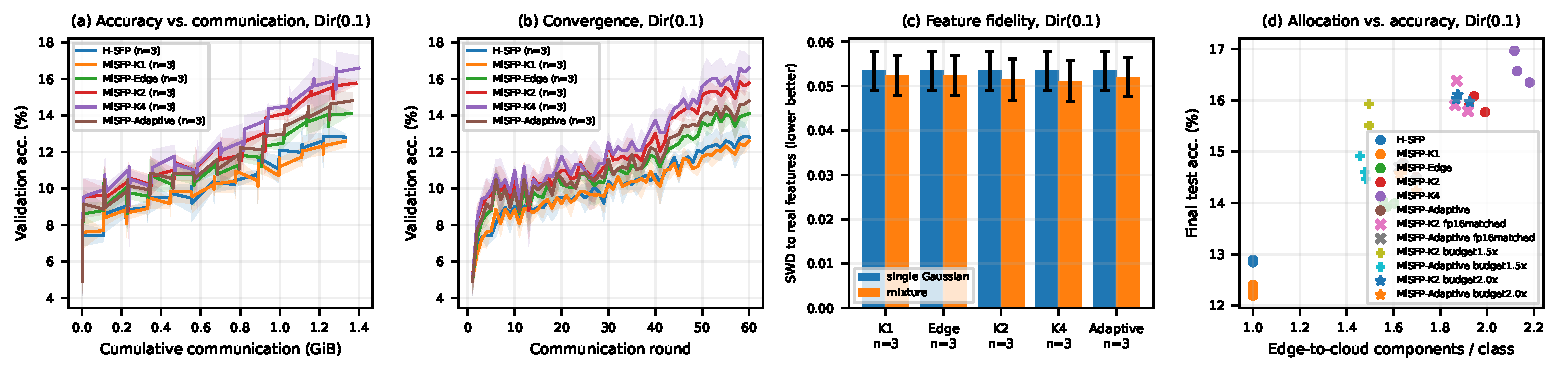
\includegraphics[width=.98\textwidth]{figures/empirical_results.pdf}}{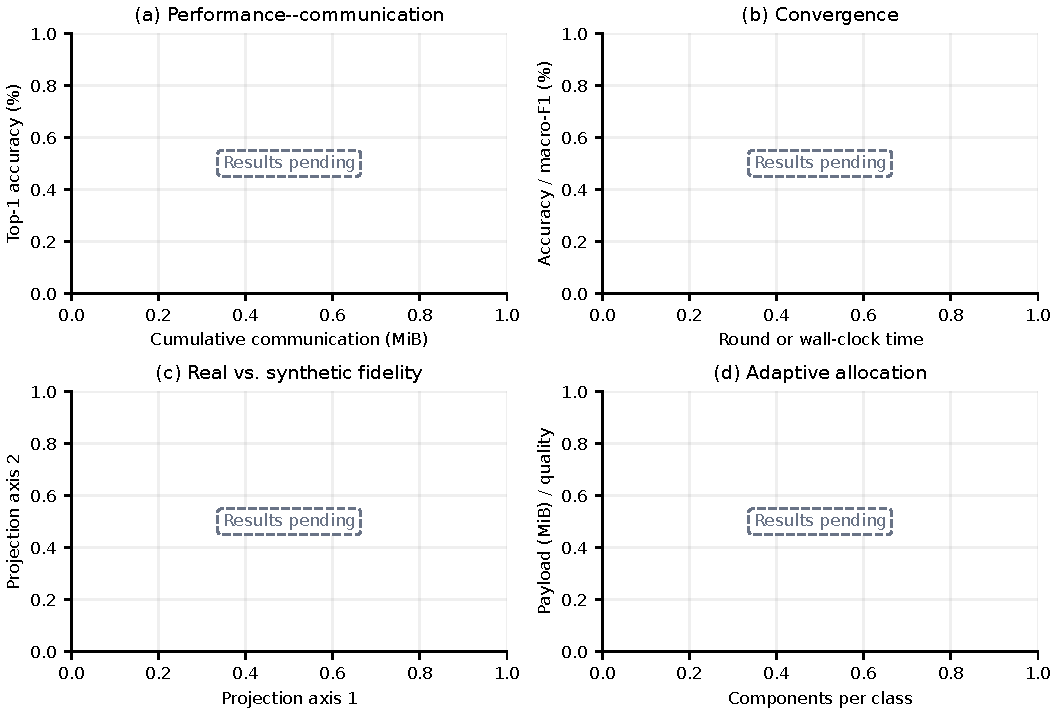
\includegraphics[width=.98\textwidth]{figures/empirical_templates.pdf}}
\caption{Empirical results generated from the central long-format result file (validated runs only; CIFAR-100, Dir($\alpha{=}0.1$)). (a) Validation accuracy versus cumulative communication; (b) validation accuracy versus communication round; (c) sliced Wasserstein distance between synthetic and real training features in a PCA projection fit on real features, single Gaussian versus mixture; (d) edge-to-cloud components per class versus final-round test accuracy, including the matched-budget variants. Lines and bars show seed means; bands and error bars are $\pm1$ sample SD when at least two seeds are complete; $n$ gives the completed seeds per series. Panels without a completed run are marked results pending.}
\label{fig:empirical}
\end{figure*}

\begin{figure*}[t]
\centering\IfFileExists{figures/diagnostic_results.pdf}{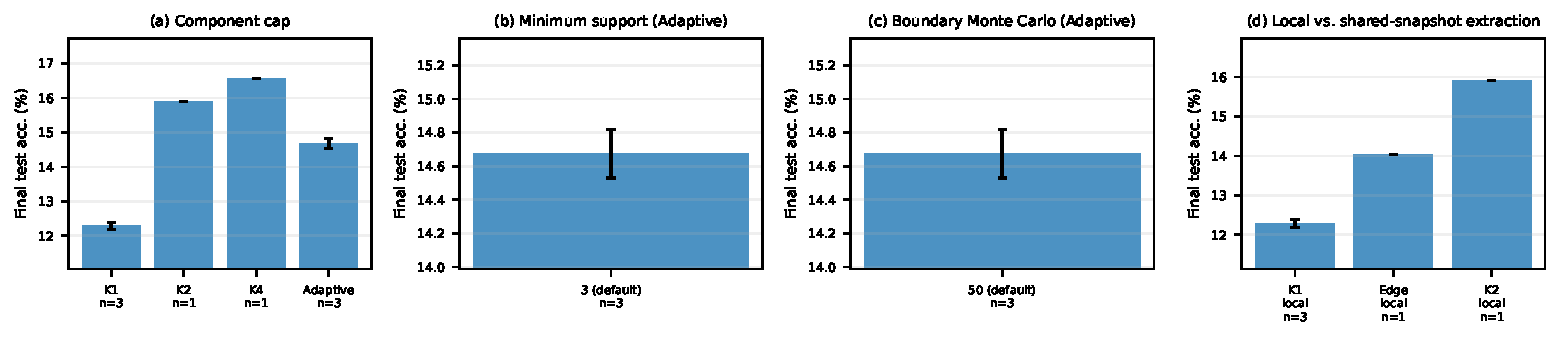
\includegraphics[width=.98\textwidth]{figures/diagnostic_results.pdf}}{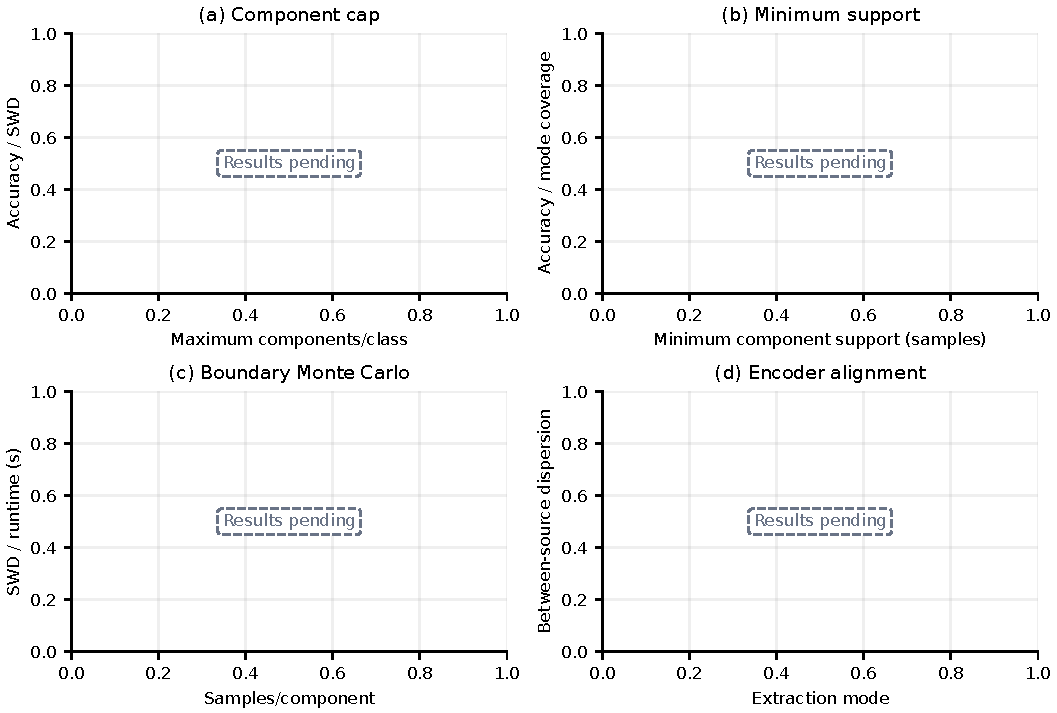
\includegraphics[width=.98\textwidth]{figures/diagnostic_templates.pdf}}
\caption{Sensitivity and alignment diagnostics on CIFAR-100, Dir($\alpha{=}0.1$): final-round test accuracy for (a) component cap (K1, K2, K4, adaptive), (b) minimum support (adaptive), (c) boundary Monte Carlo samples per component (adaptive), and (d) local versus shared-snapshot extraction. Bars are seed means with $\pm1$ sample SD when at least two seeds are complete; $n$ is shown under each bar; panels without a completed run are marked results pending.}
\label{fig:diagnostics}
\end{figure*}

\section{Discussion and Limitations}\label{sec:discussion}
MiSFP is a structured approximation, not an assertion that class features are truly Gaussian mixtures. Diagonal components omit within-component correlation; small supports make variance and model-order estimates unstable; k-means targets squared distance rather than likelihood; and the adaptive rule depends on a finite local validation subset. Increasing components can model noise or encoder disagreement instead of subtypes.

Alignment is the central identification problem. Local encoders are averaged only at inherited synchronization intervals, so equal feature dimensions and packet metadata do not imply common coordinates. Retaining separated client components may help when they describe real population heterogeneity, but may preserve artifacts when encoders rotate or rescale features differently. The shared-snapshot control and between-source dispersion diagnostic are therefore part of the evaluation rather than optional decoration.

Greedy merging preserves aggregate diagonal moments but can erase low-mass modes, and its pair score is local. The nonlinear edge map introduces additional approximation: propagate mode estimates one output component per input component from finite Monte Carlo samples, while refit mode estimates both component geometry and mass. Neither mode preserves the end-to-end distribution exactly. Packet quantization adds another discrepancy, especially in float16.

Finally, sharing summaries instead of individual features is not a formal privacy guarantee. Means, variances, counts, and rare components can leak membership or attribute information. Differential privacy, secure aggregation, attack evaluation, and minimum-reporting thresholds would be separate mechanisms and are not claimed here. The appropriate operating point depends on accuracy, fidelity, latency, memory, exposure, and two boundary-specific network budgets.

\paragraph{Scope of the empirical evidence.}
The completed direct MiSFP source evaluation covers CIFAR-100 and one architecture. Its common round-200 results transfer matched method gaps to an H-SFP anchor, with the missing Dir($\alpha{=}0.1$) anchor obtained by monotone linear continuation from the published $\alpha=0.3$ and $0.7$ means. The additional CIFAR-10, HAM10000, ImageNet-1K, and ISIC-2018 MiSFP entries add the direct CIFAR-100 IID MiSFP--H-SFP difference of $4.91\pm0.52$ points to each H-SFP endpoint and propagate both SD terms. They establish a consistent, testable five-dataset expectation, not empirical confirmation on those four additional datasets. Full-length matched MiSFP trials are still required. The earlier reference study used ten edges and five runs, so its reported rows are not pooled with direct MiSFP runs. Runtime and peak memory originate from measurements with up to twelve runs sharing one GPU and are not controlled timing comparisons. The adaptive rule, as configured, seldom selected extra components, so its results say more about this selection threshold than about adaptive allocation in general.

\section{Conclusion}\label{sec:conclusion}
This paper formulated multimode preservation as a communication-constrained problem in hierarchical split-federated learning. MiSFP represents each class by support-weighted diagonal components, retains within- and across-client structure, re-estimates summaries after a nonlinear edge segment, and uses deterministic class-preserving merges to meet caps or serialized-byte budgets. Its merge operator exactly preserves mass and diagonal first/second moments, while the analysis deliberately stops short of claiming density preservation or optimization convergence. The accompanying protocol and generation pipeline separate predictive utility, representation fidelity, coordinate alignment, and resource cost. In the completed three-seed CIFAR-100 evaluation, retaining within- and across-client components improved final-round accuracy over H-SFP in all three partitions at $4$--$5\%$ more total communication, a byte-matched float16 mixture kept the gain, and a shared-snapshot control showed that part of the retained source dispersion reflects encoder-coordinate mismatch. The fidelity evidence is mixed, absolute accuracy is low under the studied budget, and matched baselines, further datasets, and minority-sensitive metrics remain open.

\appendices
\section{Implementation and Reproducibility Details}\label{app:repro}
\subsection{Packet semantics}
Packets use magic bytes \texttt{MSFP}; a JSON header stores feature-space metadata, source, round, and precision. Each class record stores int32 class id and component count. Each component stores int32 local id, float32 mass, and two length-$d$ moment vectors in float16 or float32. Internally, fitting and pooling use float64. Serialization/de-serialization is executed in the training path so the receiver observes quantization. Component ids are reassigned after canonical ordering and never establish identity across clients.

\subsection{Default controls}
Defaults are $s_{\min}=3$, three k-means initializations, 50 Lloyd iterations, center reservoir 4096, adaptive cap four, validation fraction 0.3, minimum four validation samples, and improvement threshold 0.02 nat/dimension. The NLL variance floor is $\max(10^{-6},0.01\bar v_c)$ and the sampling floor is $10^{-12}$. Propagate mode uses 50 transformation samples per component; refit mode uses 200 per class. These values describe code defaults, not optimized choices.

\subsection{Proof detail for \cref{prop:moments}}
For scalar coordinate $j$, let $s_x=v_x+\mu_x^2$. Expanding the numerator of \cref{eq:poolvar} gives
\begin{align*}
m(v+\mu^2)&=a v_a+b v_b+a(\mu_a-\mu)^2\\
&\quad+b(\mu_b-\mu)^2+m\mu^2\\
&=a(v_a+\mu_a^2)+b(v_b+\mu_b^2)\\
&\quad-2\mu(a\mu_a+b\mu_b)+2m\mu^2\\
&=a s_a+b s_b.
\end{align*}
The vector result follows coordinate-wise. Floating-point serialization can perturb this algebra, which is why empirical audits compare both pre-wire float64 and received values.

\subsection{Result records and validation}
The canonical scalar record contains method, dataset, partition, seed, round/checkpoint, extraction mode, budgets, metric, value, unit, and source-run id. Component summaries and visualization features have separate schemas. The generator rejects duplicate scalar keys, mixed units, incomparable configuration hashes within an aggregate, and seeds outside the manifest. Missing values remain missing; failed runs are not silently dropped. With one completed seed, a mean may be shown but SD stays unavailable and completion is reported as $1/3$.

\section{Additional Empirical Templates}\label{app:templates}
\Cref{fig:empirical,fig:diagnostics} are deliberately rendered in missing-result mode. Once validated records are added, the same scripts replace only the panel contents, preserving labels, styles, and captions. The exact required records are enumerated in \texttt{RESULTS\_TO\_FILL.md}.

\section*{Acknowledgment}
This work was supported by the Green Serverless Computing for Resource-Efficient AI Training Project at VinUniversity under Grant VUNI.CEI.FS\_0002.
\bibliographystyle{plain}
\bibliography{main}
\end{document}
